\newpage

\subsection{Sistema de procesamiento de datos $s_2$}

Para que el sistema pueda tomar decisiones por si mismo  es necesario que pueda leer el estado de los parámetros internos durante el proceso de compostaje. Según la figura \ref{fg:ArchFis} que describe la arquitectura física del sistema, se requiere el diseño de un módulo especial de adquisición de señales, módulos de acondicionamientos de señales y módulos de comunicación interna. 

\subsubsection{Adquirir los datos $M_{21}$}

En este módulo del sistema, se realiza la lectura de las sensores para las diferentes variables físicas que se van a observar durante el funcionamiento del sistema de compostaje. En esta parte se analiza y se selecciona el sensor que más se adapta a las necesidades. 

\textbf{Sensor de temperatura}

Para medir de temperatura se considero encontrar un dispositivo que funcione bajo ambientes corrosivos, que se pueda integrar a la tarjeta de desarrollo y que sea accesible. Con estos requisitos se optó por utilizar el sensor electrónico de semiconductor.

%Dentro de las desventajas, se encuentra que diversos sensores pueden sufrir perturbaciones en la composición de sus componentes conforme se exponen a temperaturas más altas, además de que muy poco empaquetados con capaces de resistir en ambientes tan corrosivos, como el que se plantea tener al interior del contenedor. 

Dentro de una lista de dispositivos comerciales,  se seleccionó el sensor DS18B20, este sensor está hecho a base de semiconductores. Este sensor esta integrado dentro del entorno de desarrollo de Arduino, por lo que su integración con la ESP 32 esta garantizada.

Otra ventaja, es que este sensor cuenta con una versión sumergible, que posee una cubierta  impermeable de acero inoxidable, de esta manera el sensor puede trabajar bajo condiciones de humedad que no afectan su funcionamiento, además de protegerlo de la corrosión.  Los detalles técnicos del sensor son los que describen en la tabla \ref{tab:Sensortem}

\begin{table}[h!]
    \centering
    \caption{Características del sensor DS18B20}
        \begin{tabular}{ |c|c|c|c| } 
            \hline
            \multirow{7}{8em}{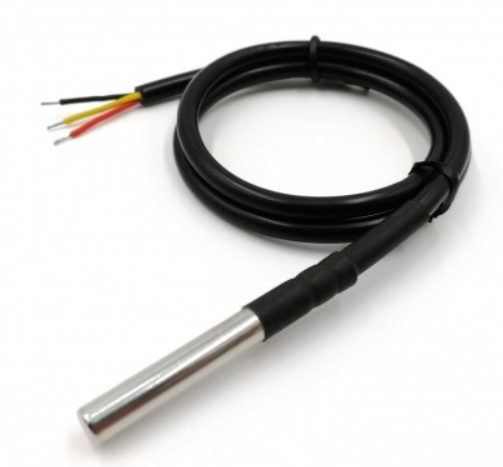
\includegraphics[scale=0.15]{images/Capitulo 4/S2/temperatura.png}} & \cellcolor[rgb]{ .851,  .851,  .851}Alimentación & \cellcolor[rgb]{ .851,  .851,  .851}3.0 a 5 V \\ 
            & Resolución & 9 a 12 bit \\ 
            & \cellcolor[rgb]{ .851,  .851,  .851}Rango de temperatura & \cellcolor[rgb]{ .851,  .851,  .851}50 a 125 C \\ 
            & Diámetro de la probeta & 6 a 9 mm \\
            & \cellcolor[rgb]{ .851,  .851,  .851}Largo de la probeta & \cellcolor[rgb]{ .851,  .851,  .851}10 a 1000 mm \\
            & Material de la probeta & Acero inoxidable \\
            & \cellcolor[rgb]{ .851,  .851,  .851}Conector & \cellcolor[rgb]{ .851,  .851,  .851}Molex, DuPont, CWB, CJT, U type\\
             \hline
        \end{tabular}
    \label{tab:Sensortem}%
\end{table}

\textbf{Sensor de humedad}

Para la medición de la humedad, se tomaron en cuenta dos tipos de sensores, los sensores que tienen contacto con la materia orgánica y los sensores que miden la humedad del ambiente. Para efectos de este trabajo, se ha seleccionado el sensor que mide la humedad del ambiente dentro del tanque del compostador.

Para esta parte se optó por utilizar el sensor de humedad y temperatura DHT11, este es un sensor electrónico que capta la humedad del ambiente y es capaz de mandar una señal digital con toda la información que ha captado. 

Este dispositivo también cuenta con una librería en el entorno de desarrollo de arduino, por lo que su integración con la tarjeta de desarrollo esta garantizada, además de que es un dispositivo económico, que según los antecedentes revisados en la tabla \ref{tab:Antecedentes}, tiene buen desempeño en este tipo de sistemas de compostajes. 

Las características del sensor, aparecen en la tabla \ref{tab:Sensorhum}

\begin{table}[h!]
    \centering
    \caption{Características del sensor DHT11}
        \begin{tabular}{ |c|c|c|c| } 
            \hline
            \multirow{6}{8em}{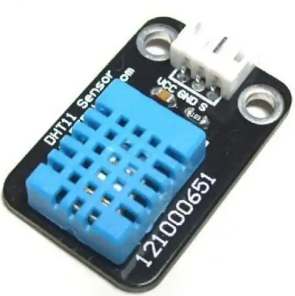
\includegraphics[scale=0.25]{images/Capitulo 4/S2/Humedad.png}} & \cellcolor[rgb]{ .851,  .851,  .851}Alimentación & \cellcolor[rgb]{ .851,  .851,  .851}3.0 a 5.5 V \\ 
            & Resolución & 1\% a 8 bit \\ 
            & \cellcolor[rgb]{ .851,  .851,  .851}Rango de humedad & \cellcolor[rgb]{ .851,  .851,  .851}20 a 80 \% \\ 
            & Tiempo de respuesta & 6 a 10 s \\
            & \cellcolor[rgb]{ .851,  .851,  .851}Señal de salida & \cellcolor[rgb]{ .851,  .851,  .851} Digital \\
            & \cellcolor[rgb]{ .851,  .851,  .851}Conector & \cellcolor[rgb]{ .851,  .851,  .851}DuPont\\
             \hline
        \end{tabular}
    \label{tab:Sensorhum}%
\end{table}

\subsubsection{Acondicionamiento de señales $M_{22}$}

Debido a cómo están configurados los sensores seleccionados, el proceso de acondicionamiento de la señal se realiza de forma digital al interior de la tarjeta de desarrollo a través de las librerías que existen en el entorno de desarrollo, por lo que el circuito electrónico es mas simple, solo se utilizaron unas cuantas resistencias, sugeridas por los proveedores que están conectadas entre la salida de datos del sensor y el pin donde estarán conectados a la tarjeta de desarrollo.

Esto se hizo con el fin de reducir las interferencias de ruido, además de provocar una caída de tensión para la lectura de los pulsos digitales. La forma en como se puede realizar su conexión en una tarjeta de desarrollo se puede ver en las figuras \ref{fg:tempacpnd} y \ref{fg:dht11acondi}

Finalmente, los sensores se integraron al esquema que se realizo para la interfaz, donde están conectados a la tarjeta ESP-32 como se muestra en la figura \ref{fg:CTO MONITOREO}



\begin{figure}[h!]
            \centering
            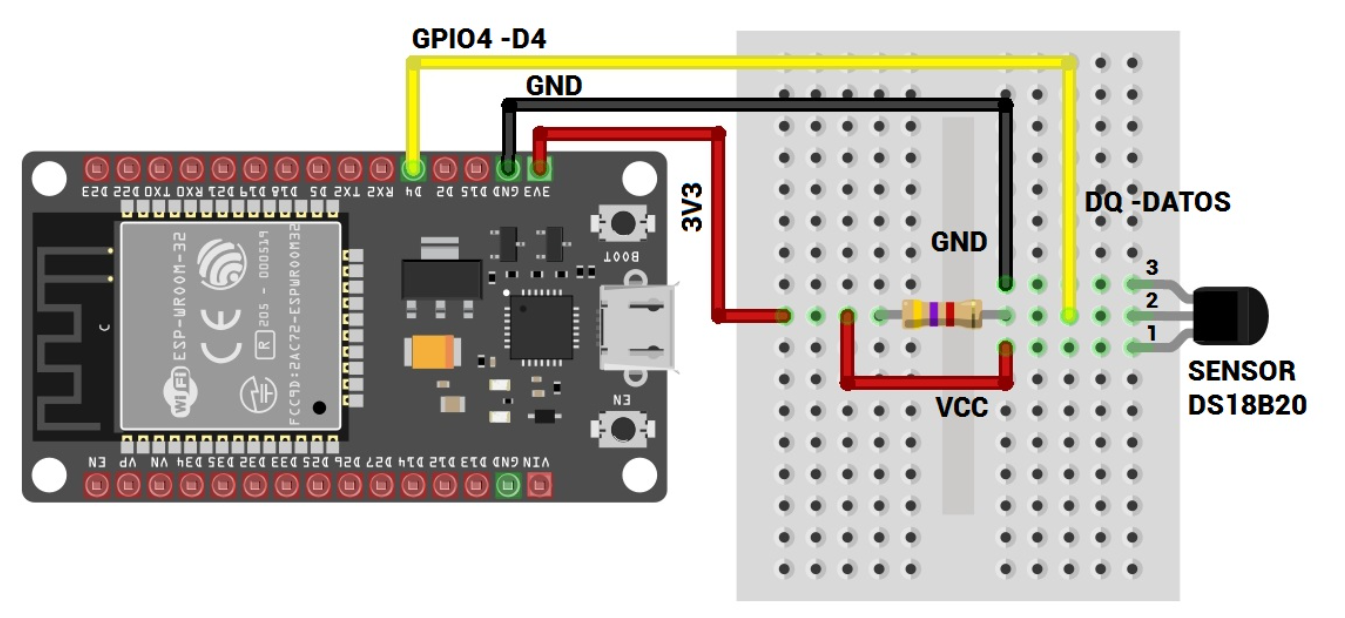
\includegraphics[scale=0.25]{images/Capitulo 4/S2/tempacons.png}
            \caption{Ejemplo de conexión del sensor DS18B20 a una tarjeta de desarrollo \cite{TempSensor}}
            \label{fg:tempacpnd}
        \end{figure}

\begin{figure}[h!]
            \centering
            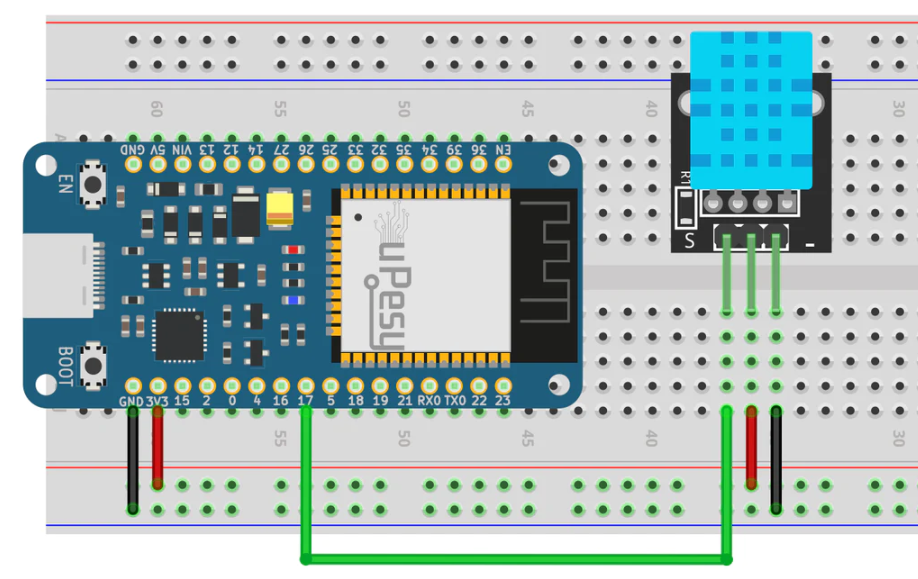
\includegraphics[scale=0.25]{images/Capitulo 4/S2/DHT11ACON.png}
            \caption{Ejemplo de conexión del sensor de humedad DHT11 a una tarjeta de desarrollo \cite{DHT11acon}}
            \label{fg:dht11acondi}
        \end{figure}

\begin{figure}[h!]
            \centering
            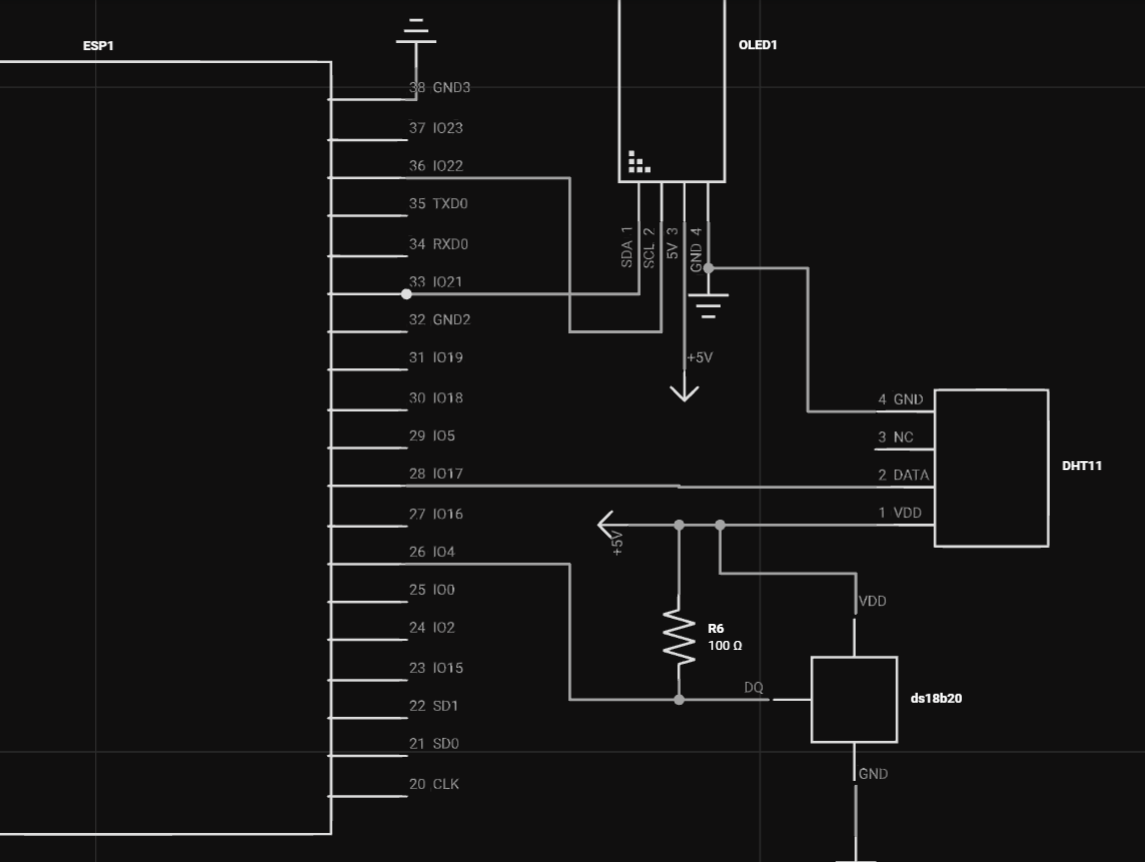
\includegraphics[scale=0.25]{images/Capitulo 4/S2/CTO Monitoreo.png}
            \caption{Integración de los sensores en la tarjeta de desarrollo}
            \label{fg:CTO MONITOREO}
        \end{figure}


\newpage

\subsubsection{Comunicación interna $M_{23}$}

Por medio de estos enlaces internos, el sistema estará intercambiando información de forma constante entre los diferentes módulos con el fin de conocer el estado del proceso y tomar decisiones para realizar las operaciones para llevar a cabo las tareas del proceso de compostaje.

Existen 3 vías de comunicación (figura \ref{fg:convia}), la primera es una vía unidireccional, la cual será la encargada de enviar toda la información que se genera al interior del recipiente de compostaje, esta información contiene el valor de la temperatura y la humedad al interior del contenedor. Con esta información, la unidad de procesamiento será capaz de tomar decisiones sobre los actuadores.

Existe otra vía de comunicación unidireccional, la cual será la encargada de realizar las interacciones de con los actuadores del sistema (Sistema de riego, Sistema de ventilación, Sistema de temperatura y Sistema de aeración). Estas señales se encargan de la activación de los actuadores después del procesamiento de la información en el controlador. 

Por último, existe una vía de comunicación bidireccional, esta vía es la Interfaz Humano - Máquina, esta vía envía los datos que se generan al interior del proceso y a su vez, recibe algunas instrucciones desde el exterior. 

Para la implementación física de estos buses de comunicación, se planteó la conexión por medio de cables dupont, los cuales estarán conectados por medio de headers que se colocaran en las PCB que se estén desarrollando para los sistemas electrónicos del sistema.

\begin{figure}[h!]
            \centering
            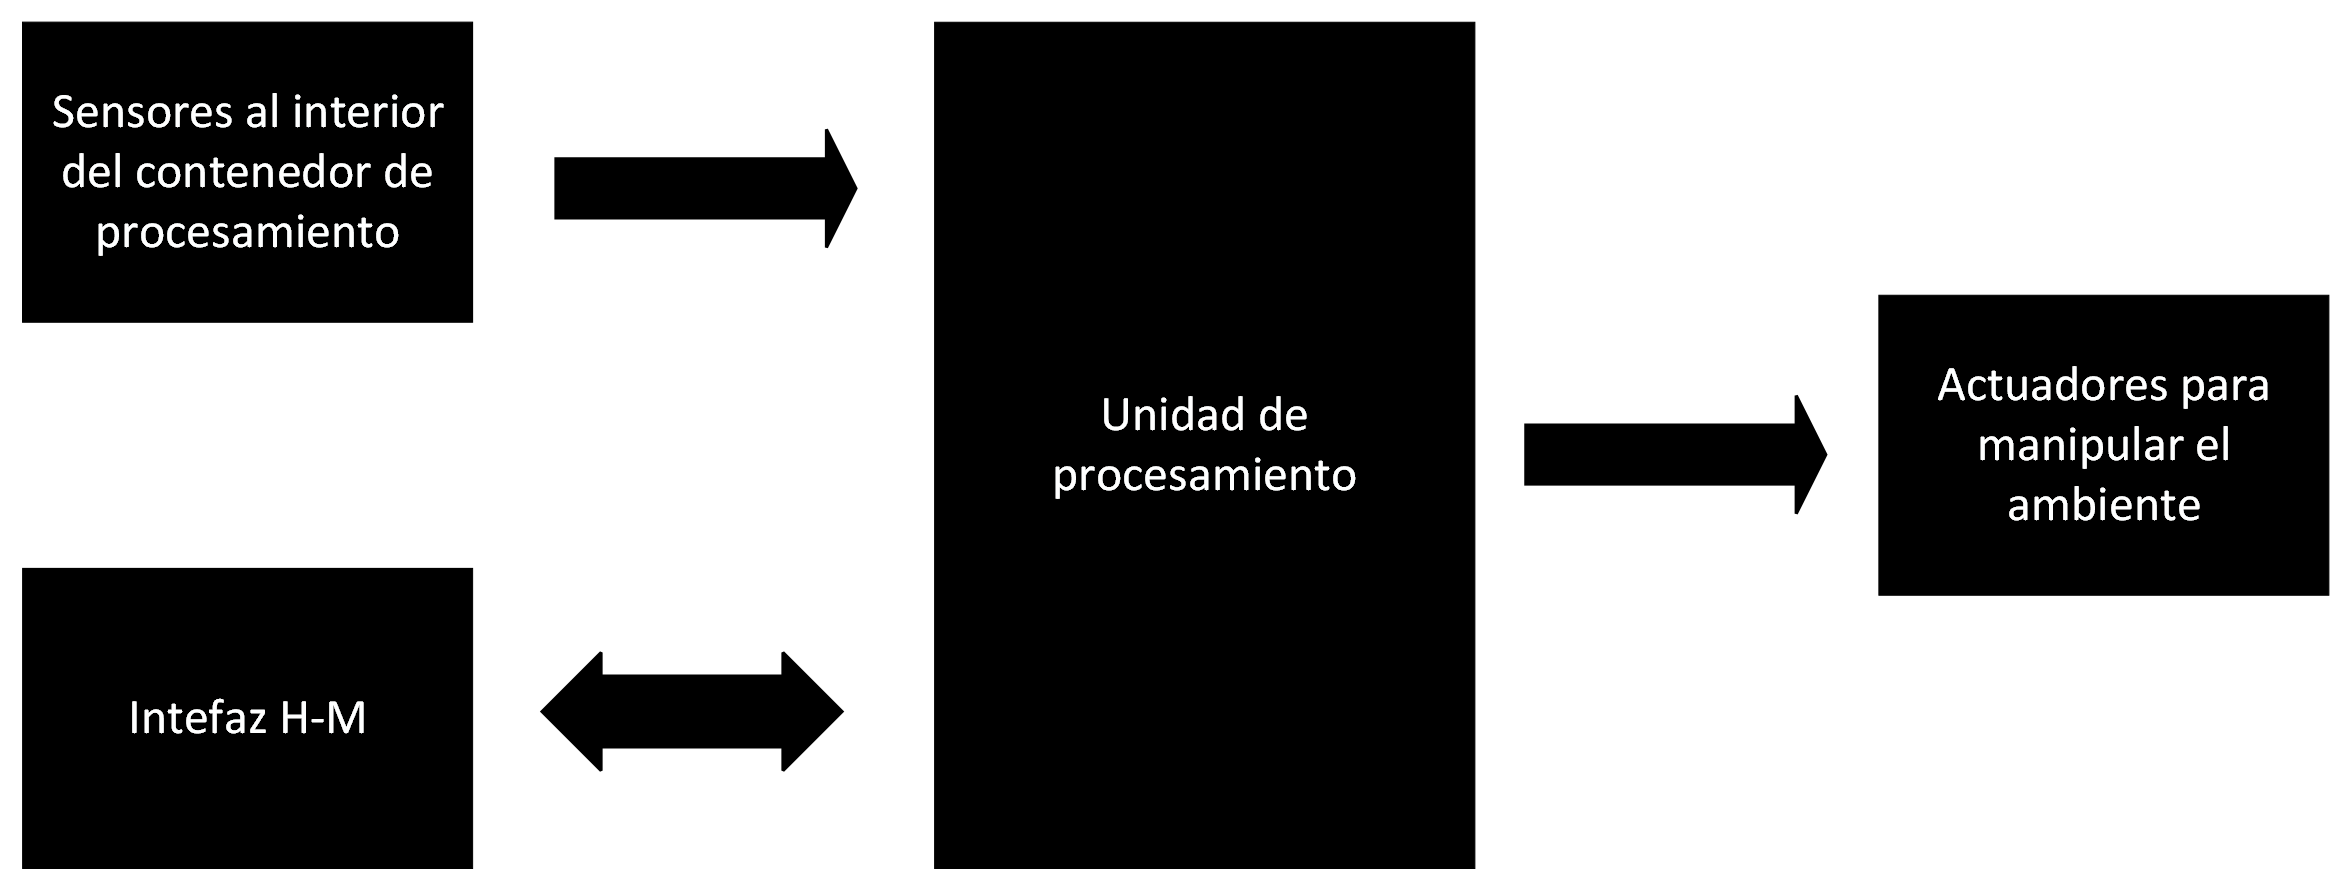
\includegraphics[scale=0.7]{images/Capitulo 4/Canales de comunicacion.png}
            \caption{Salidas y entradas de comunicación con la unidad de procesamiento}
            \label{fg:convia}
        \end{figure}
%\subsubsection{Diseño de los circuitos requeridos}

A partir de las ideas ya expresadas en los puntos anteriores, se comienza con el diseño del circuito principal del sistema. Este circuito lleva en su corazón la tarjeta ESP32, la cual será la encargada de comandar y de sincronizar todas las tareas. De igual forma, se considera como la distribución principal de la energía del sistema a los circuito con alimentación de 5V dc.

De esta forma, la placa principal, estará compuesta por la ESP32 y diversos headers que irán desde cada una de sus terminales a todos los demás módulos, por medio de cables dupont, que servirán para comunicar a todos los circuitos y sensores entre si.

En la figura \ref{fg:principal_esq} se puede ver como se pretende llevar la interconexión de cada uno de los módulos, simulando las entradas de la ESP32 y realizando las pistas en cada una de las puntas de salida a cada circuito externo, también se ve cómo sería la PCB para el funcionamiento del sistema (Figura \ref{fg:PCB_Principal})

\begin{figure}[h!]
            \centering
            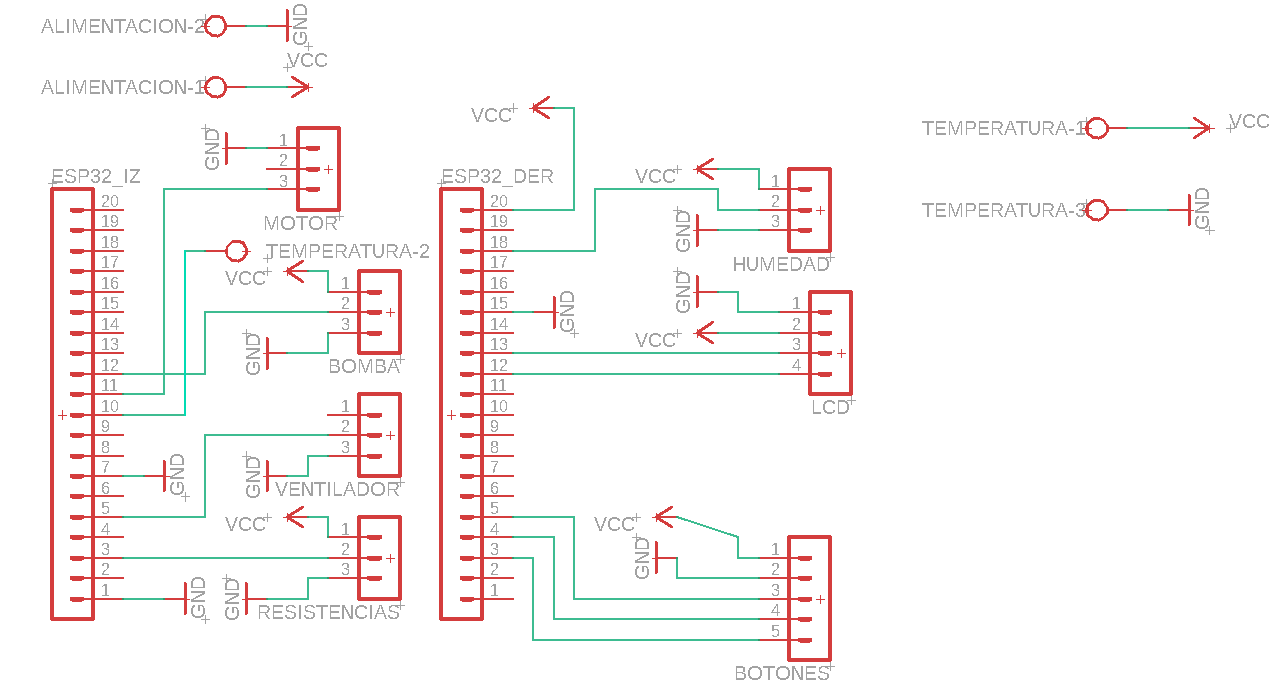
\includegraphics[scale=0.3]{images/Capitulo 4/3.1.1/principal.png}
            \caption{Circuito esquemático del cerebro del sistema}
            \label{fg:principal_esq}
        \end{figure}

\begin{figure}[h!]
            \centering
            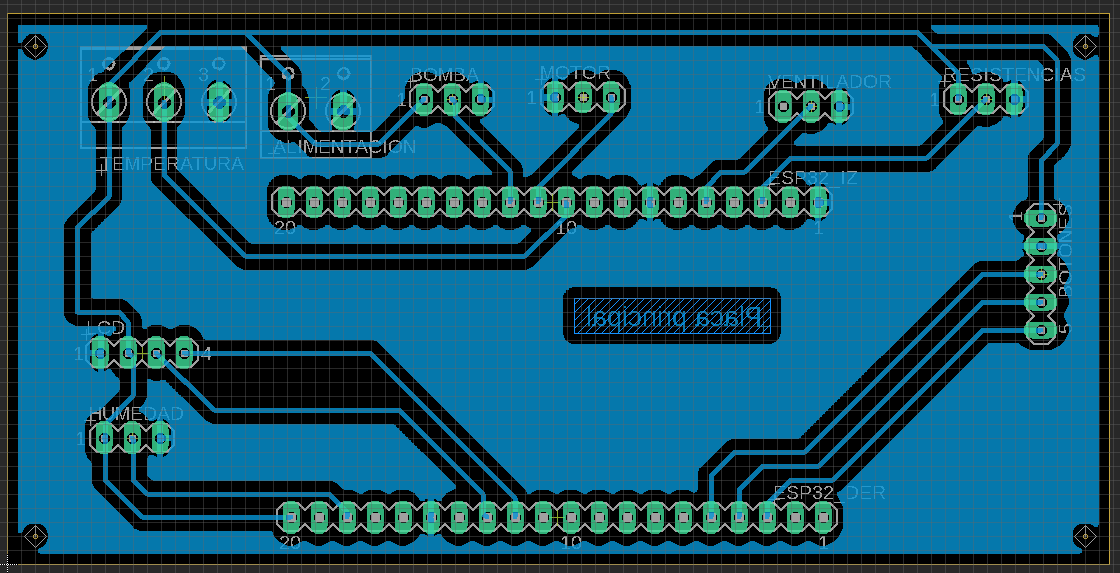
\includegraphics[scale=0.3]{images/Capitulo 4/3.1.1/Principal PCB.png}
            \caption{PCB principal del sistema}
            \label{fg:PCB_Principal}
        \end{figure}